\section{Diskussion}
Im ersten Versuchsteil ist die Funktion des Lock-In-Verstärkers deutlich zu sehen. Zwar zeigen die Spannungskurven der beiden Messreihen leicht unterschiedliche Formen auf, was möglicherweise an fehlerhaften Einstellungen
der Messgeräte liegen könnte, aber dennoch sind bei der zweiten Messreihe trotz Rauschsignal die eigentlichen, ungestörten Spannungskurven klar zu erkennen. Somit ist die Funktionsweise des Lock-In-Verstärkers
verifiziert.

Im zweiten Versuchsteil wird festgestellt, dass die Messwerte recht gut dem Abstandsgesetz entsprechen, da die meisten Werte sehr nah an der Ausgleichskurve $y = \frac{a}{(r+b)^2}$ liegen. Zu Bestimmung des maximalen Abstands
müssten allerdings mehr Werte aufgenommen werden um ein eindeutiges Ergebnis zu bekommen. Da der Versuch in einem beleuchteten Raum durchgeführt wurde, hätte eine Messung ohne Photodiode gemacht werden müssen, 
um dadurch besser abschätzen zu können, wann der maximale Abstand erreicht ist. Alternativ könnte der Versuch auch in einem abgedunkeltem Raum gemacht werden, um ausschließlich das Licht der Diode zu erfassen. 

\pagebreak
\begin{figure}[h!tbp]
	\centering
	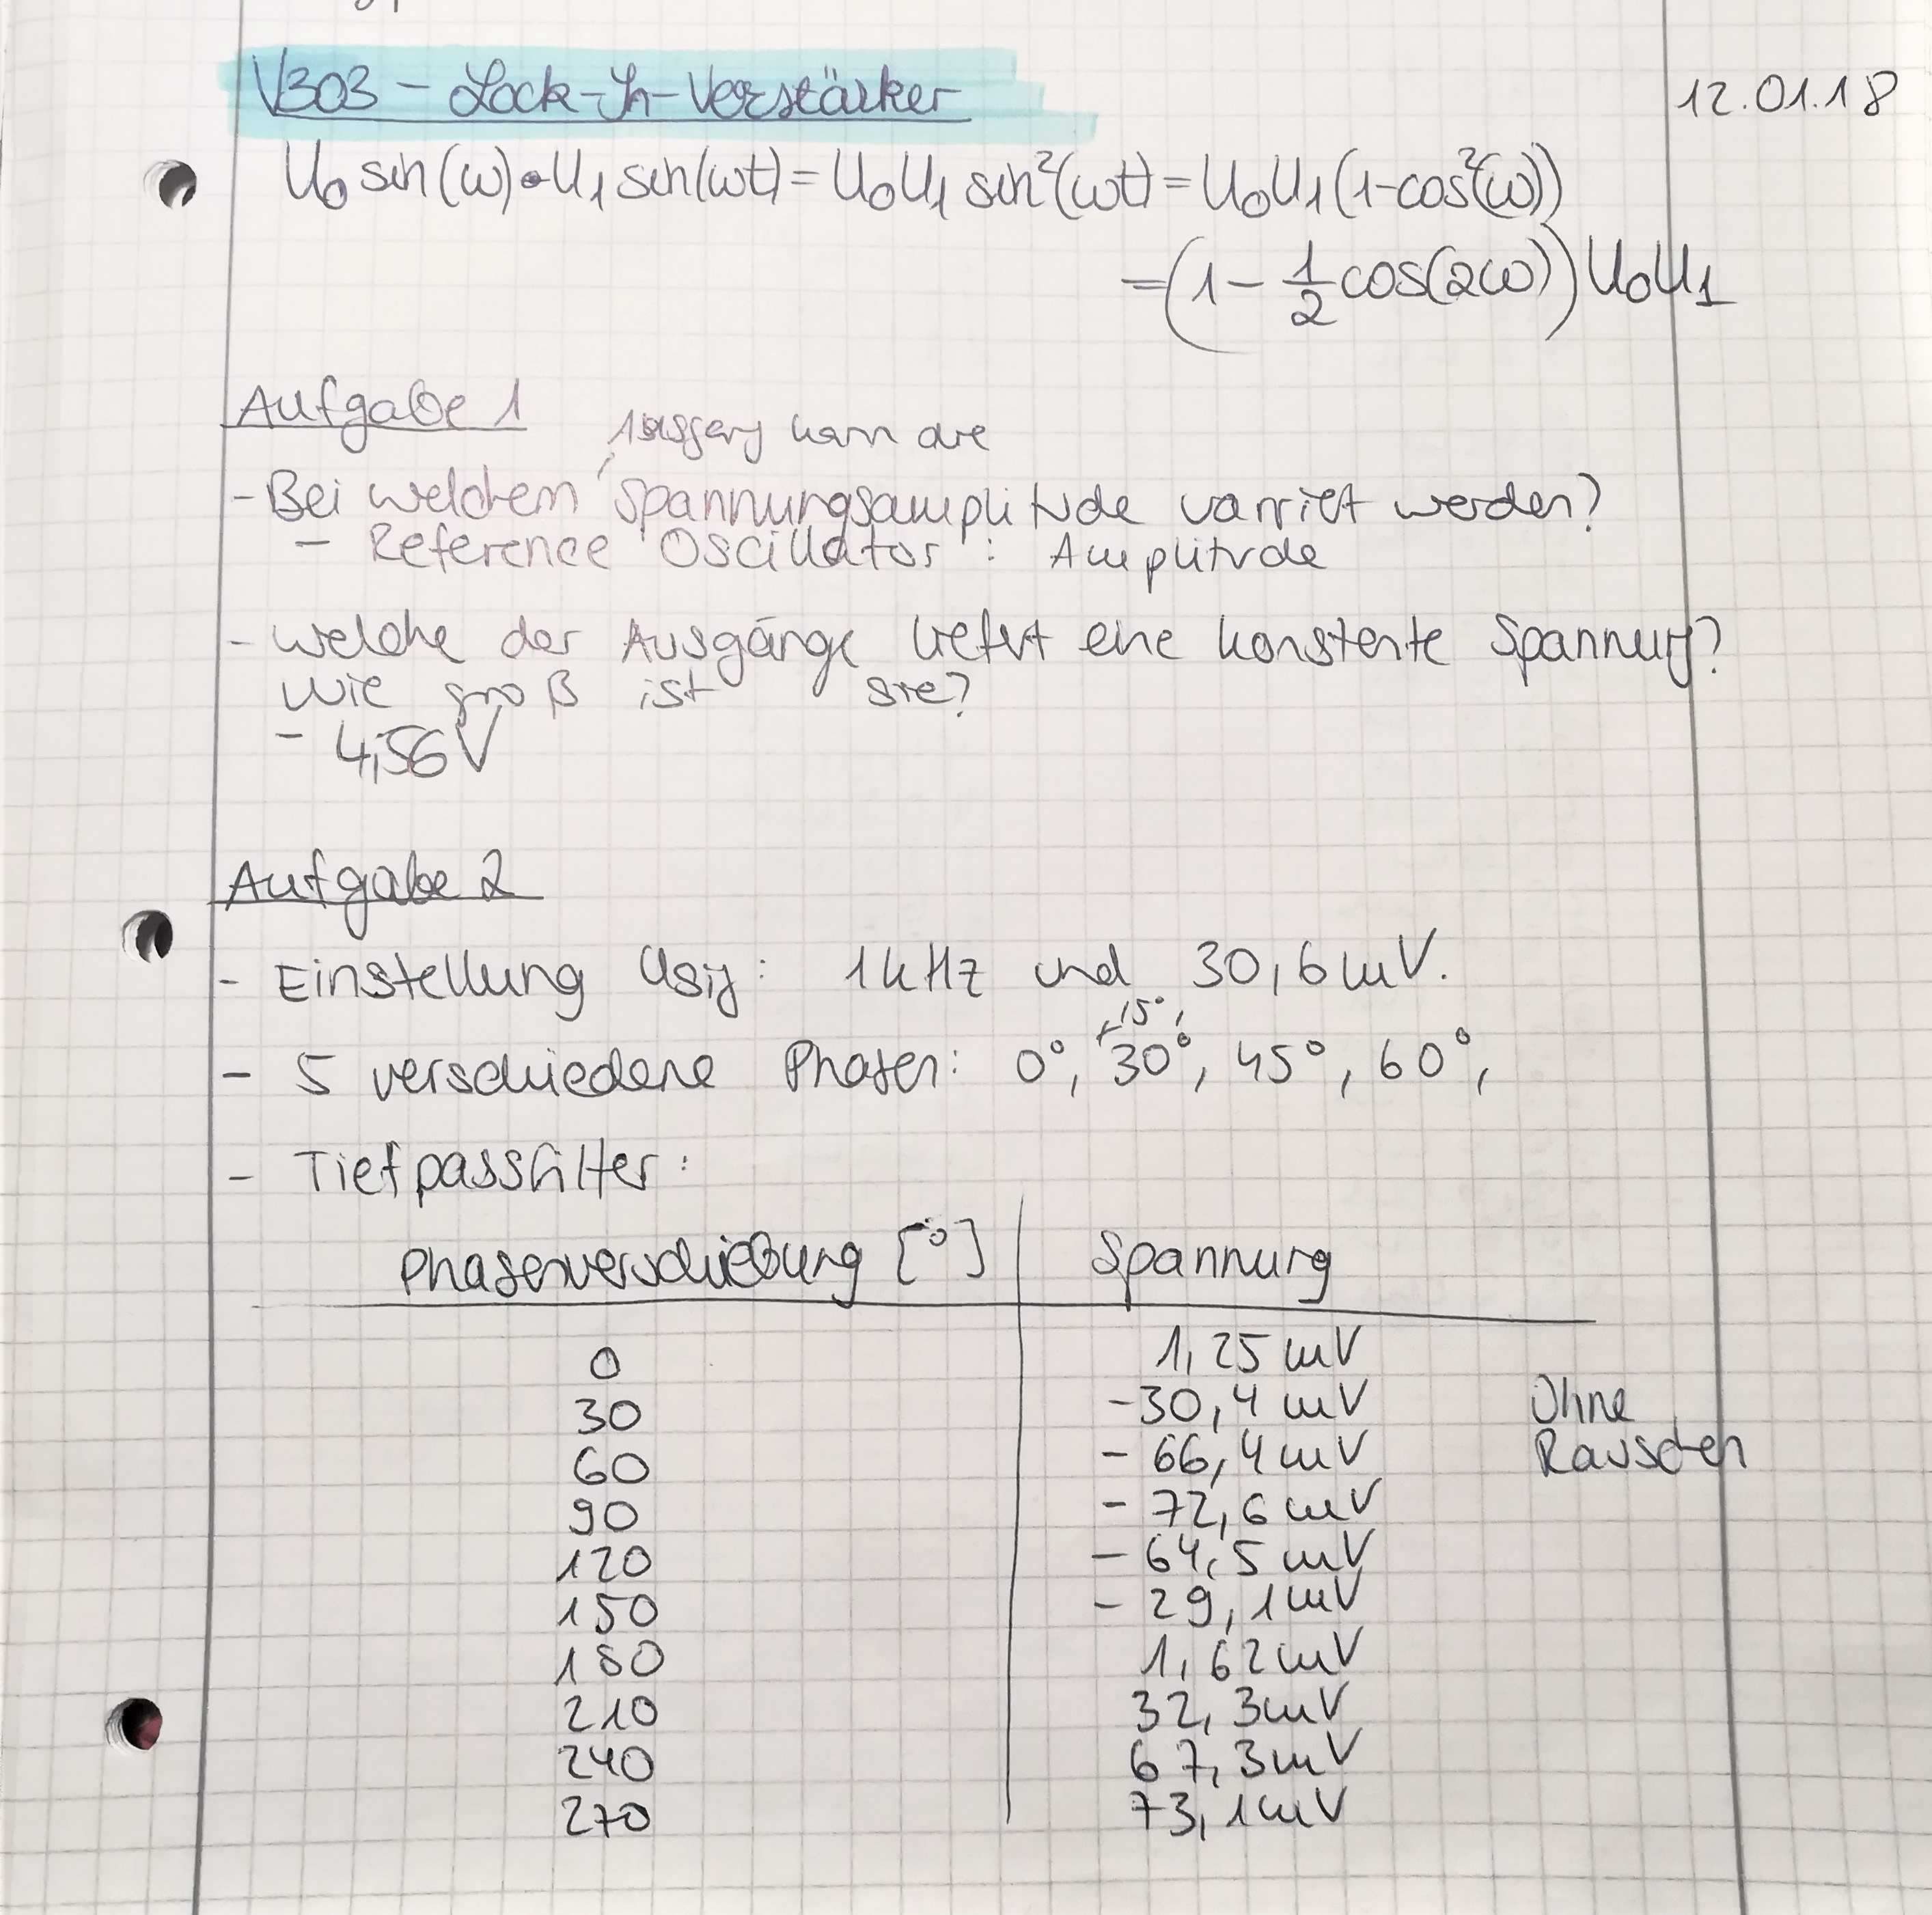
\includegraphics[width=0.9\linewidth]{Messdaten1.jpg}
	\caption{Originale Messdaten. }
\end{figure}

\begin{figure}[h!tbp]
	\centering
	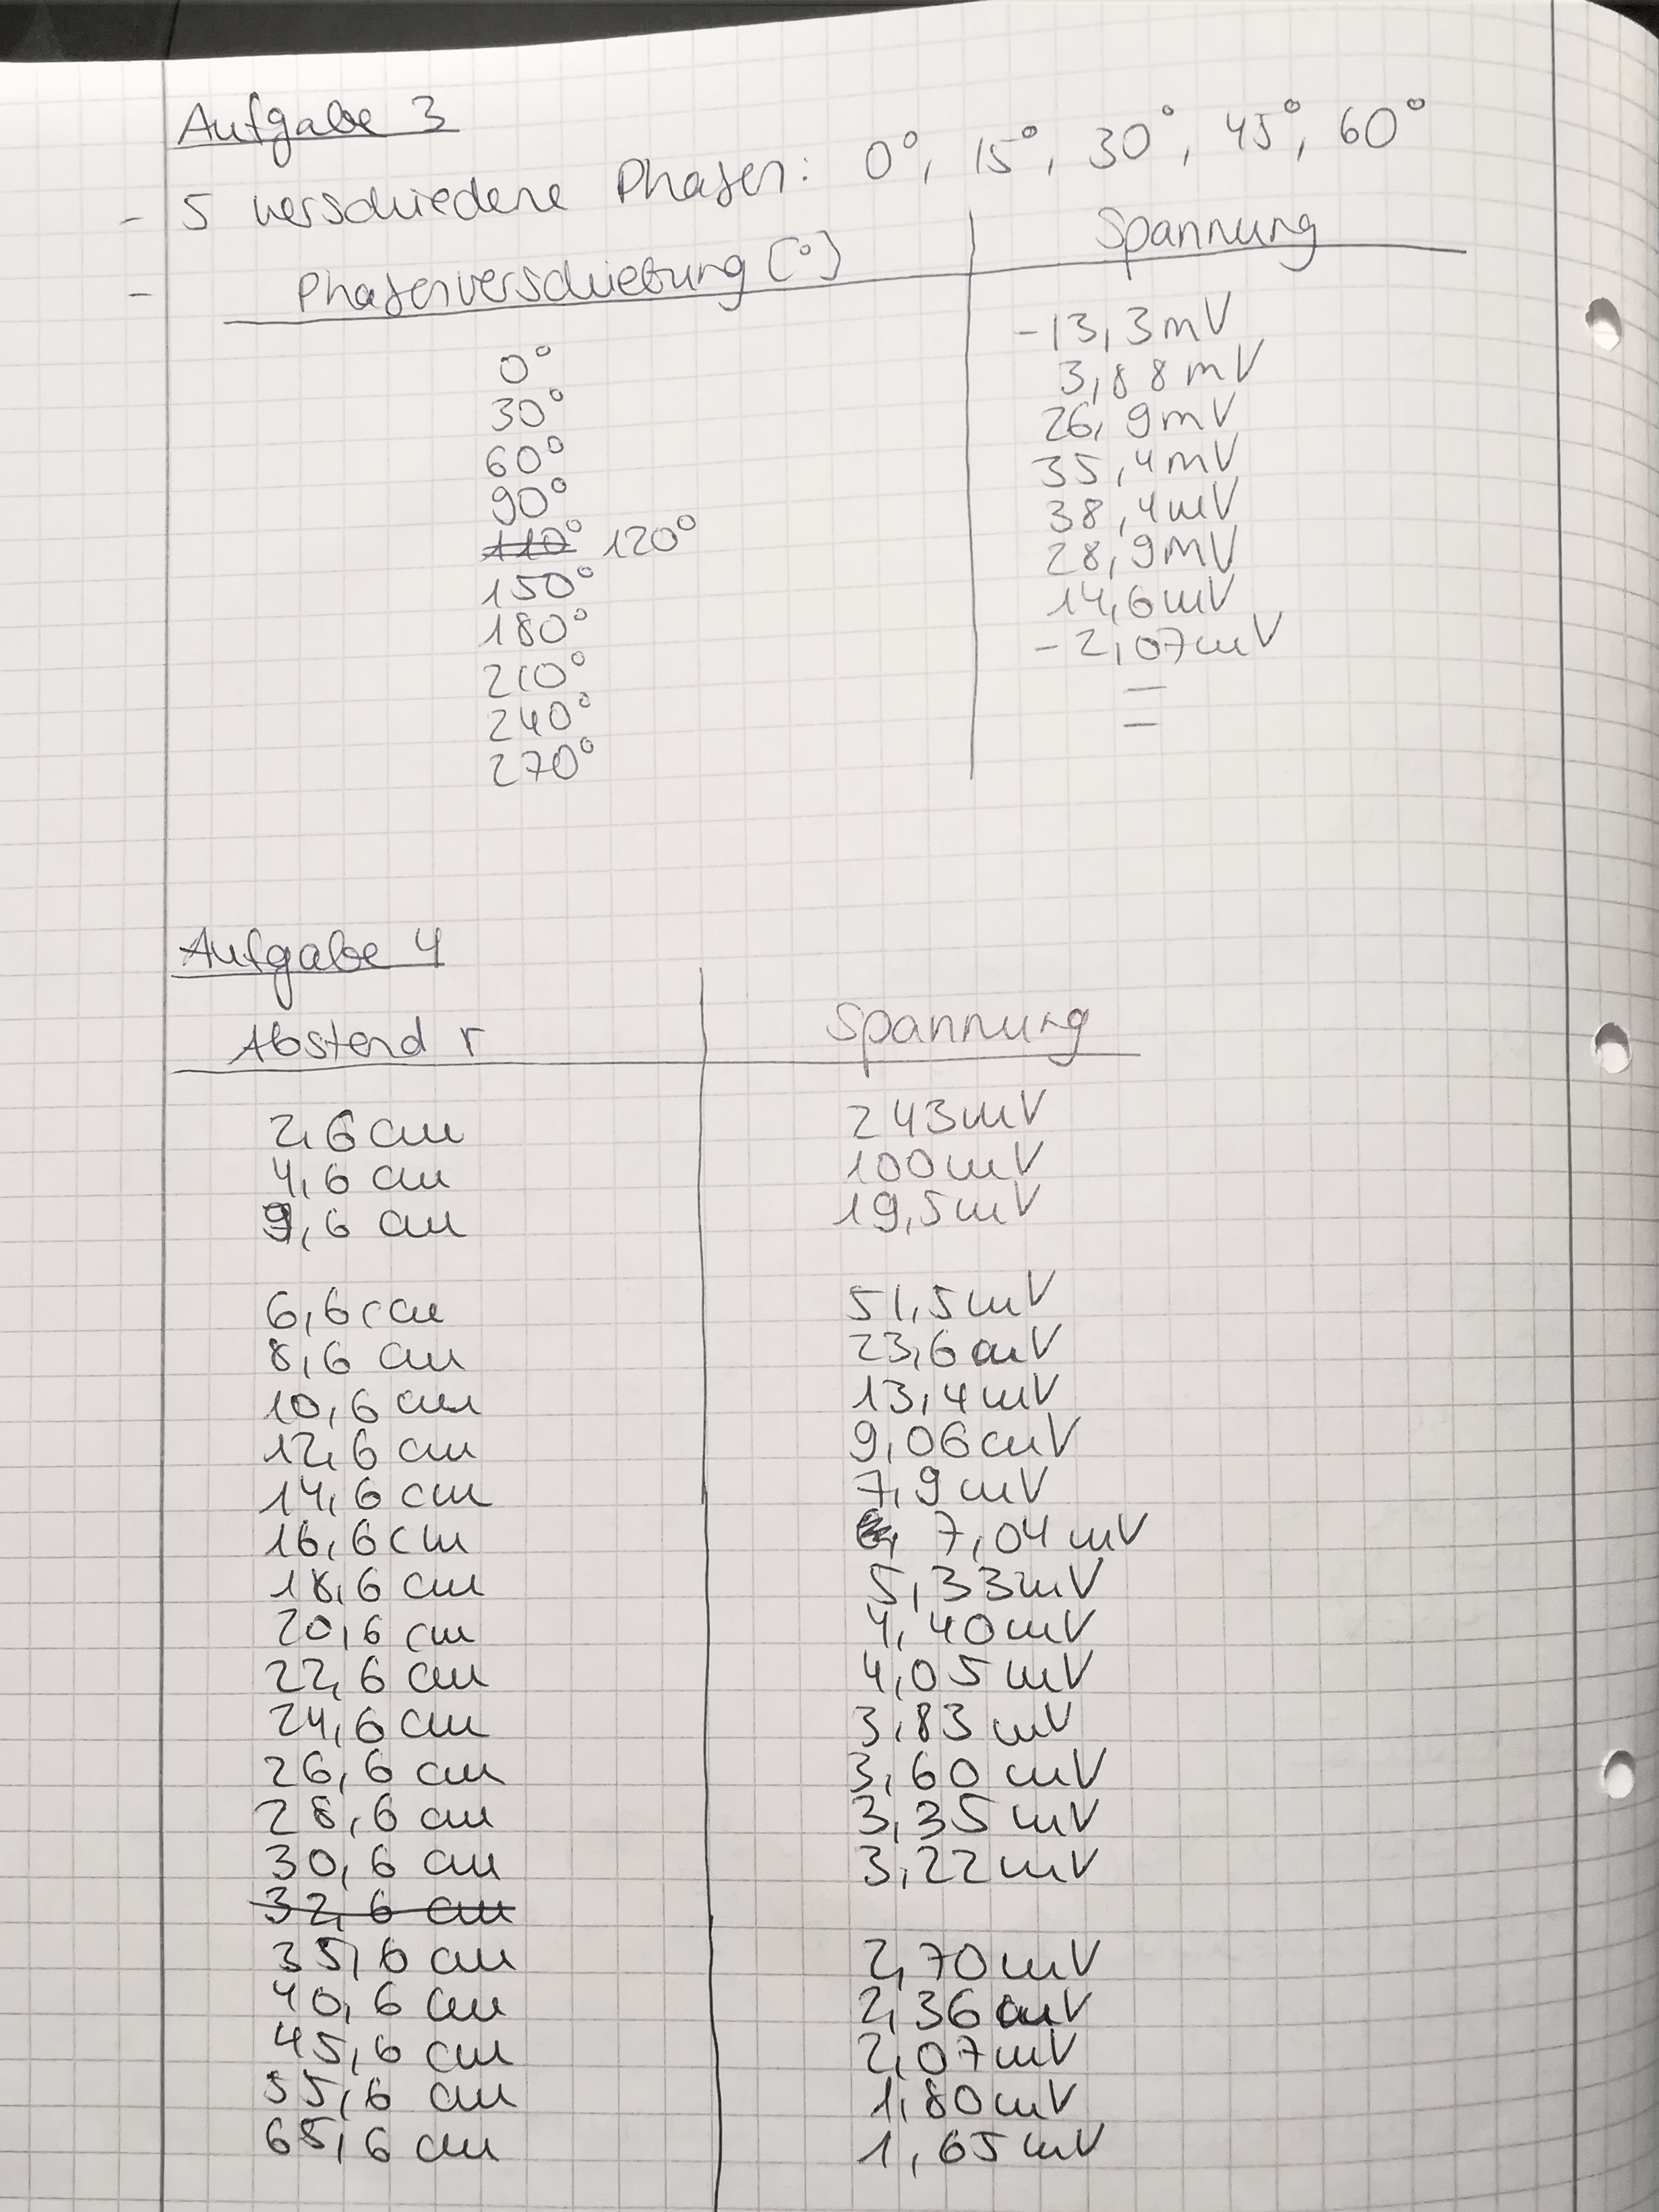
\includegraphics[width=0.9\linewidth]{Messdaten2.jpg}
	\caption{Originale Messdaten. }
\end{figure}